\chapter{Prezentacja warstwy użytkowej projektu}
Rozdział poświęcony wizualnej oraz funkcjonalnej prezentacji zrealizowanego projektu. Zanim przejdziemy do omówienia i prezentacji samych widoków witryny, warot pochylić się nad ogólnymi założeniami, które definiowały ostateczny kształt samej strony.

Głównym celem było stworzenie spójnego designu, który buduje wizerunek nowoczesnej marki.
\section{Identyfikacja wizualna i stylistyka strony}
Projekt witryny utrzymany został w estetyce ciemnego motywu jako domyślnego środowiska. Wybór ten został zrealizowany ponieważ:
\begin{itemize}
    \item \textbf{Psychologia:} Ciemne tła kojarzą się z tajemniczością jak i nowoczesną technologią co jest zmieszane, gdy tworzona była witryna.
    \item \textbf{Ergonomia:} Ciemny interfejs jest mniej męczący dla oczu, szczególnie, gdy środowisko użytkownika posiada słabe naświetlenie.
    \item \textbf{Ekspozycja treści:} Ciemne tło tworzy kontrast dla jasnych czcionek i akcentów, które pozwalają wyróżnić wyraźnie treść.
\end{itemize}
\section{Kolorystyka}
Dobór barw w projekcie nie był przypadkowy. Zastosowano minimalistyczną ilość kolorów wykorzystanych głównie z gotowych już palet na stronie \textit{\url{https://coolors.co/}}. Kolory te zostały zaimplementowane dla wielu elementów zaś one same są zdefiniowane w zmiennych \textbf{:root}. Z racji, że barwy są wykorzystywane zarówno na stronie głównej jak i podstronach tworzy to spójność na wszystkich stronach.
\begin{itemize}
    \item \textbf{Głęboka czerń (\#0A0908):} Kolor dominujący, stanowiący tło całej witryny. Nie jest to jednak czysta czerń, lecz ciemniejszy odcień szarości zaimportowany z palety koloru \textbf{Gothic Romance}.
    \item \textbf{Biel (\#F2F4F3):} Użyty jako główny tekst koloru. Zapewnia dobrą czytelność na ciemnym tle, unikając jednocześnie mocnego kontrastu.
    \item \textbf{Czerwień (\#C1121F):} Użyty jako kolor akcentujący wykorzystany głównie do elementów interaktywnych takich jak przyciski, aktywne linki oraz obramowania jak i również "logo" będące nagłówkiem \texttt{<h1>}.
    \item \textbf{Szarość (\#888888, \#222222, \#444444):} Kolory pomocnicze używane głównie do tekstów drugoplanowych oraz niekatywnych elementów takich jak ramki nienajechane kursorem.
\end{itemize}
\section{Typografia}
W warstwie typograficznej postawiono na nowoczesne kroje bezszeryfowe (Sans-Serif), importowane z biblioteki \textit{Google Fonts}. Zastosowano parowanie dwóch czcionek w celu odddzielenia nagłówków od treści bieżącej.

\textbf{Czcionka główna: Kanit}
Dla tytułów, nagłówków sekcji, treści oraz haseł marketingowych zastosowano czcionkę \textbf{Kanit}. Wykorzystano wysokie wagi chociażby Bold 700 co nadaje siły i charakteru.

\textbf{Czcionka poboczna: Montserrat}
Dla menu nawigacyjnego, przycisków oraz dłuższych bloków zastosowano czcionkę \textbf{Montserrat}. Ma ładny i neutralny styl i stanowi doskonałe tło dla bardziej wyrazistej czcionki \textbf{Kanit}.

\section{Układ i kompozycja interfejsu}
W strukturze wizualnej zastosowano duże marginesy (paddigni rzędu 10rem) oraz duże odstępy między sekcjami, aby interfejs wydawał się lekki i przejrzysty, mimo iż użyte zostały ciężkie barwy. Pozwala to użytkownikowi przyswajać treści bez poczucia przytłoczenia nimi. Układ elementów zaprojektowano w oparciu o naturalne wzroce skanowania wzrokiem w osi Z, prowadząc użytkownika od nagłówka przez grafiki aż do przycisków. "Piękne" strony internetowe bardzo często są niepraktyczne gdyż użytkownik potrzebuje tylko kilku sekund aby zadecydować czy pozostać na stronie czy też nie. Stąd bardzo często stosuje się chociażby tak zwaną sekcję "hero". 

\section{Strona główna}
Strona główna pełni rolę wizytówki firmy. Zastosowano tutaj klasycznie układ blokowy zaczynając od prezentacji marki aż do szczegółów i kontaktu.
\subsection{Hero Banner}
Pierwszym elementem widocznym dla użytkownika jest sekcja Hero. Sekcja ta przedstawiona jest na rysunku poniżej - {rys. \ref{rys 5.1}}
\begin{figure}[ht!]
    \centering
    \includegraphics[width=\linewidth]{figures/5.1.eps}
    \caption{Sekcja Hero Banner witająca użytkownika}\label{rys 5.1}
\end{figure}
\subsection{Pasek nawigacji}
Pasek nawigacji (header) został zaprojektowany w minimalistyczny sposób, gdzie "logo" umieszczone jest po stronie lewej zaś załączniki po stronie prawej. Pasek nawigacji przedstawiony na rysunku poniżej - {rys. \ref{rys 5.2}}
\begin{figure}[ht!]
    \centering
    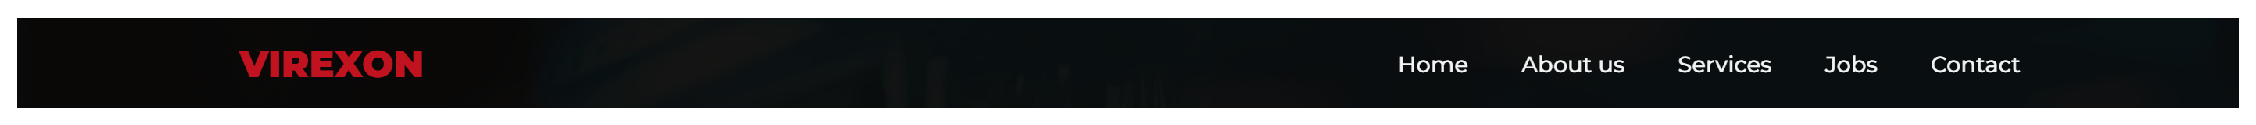
\includegraphics[width=\linewidth]{figures/5.2.eps}
    \caption{Pasek nawigacyjny}\label{rys 5.2}
\end{figure}
\subsection{Sekcja treści}
Główna część strony która wykorystuje układ naprzemienny, gdzie treść przeplata siez grafikami. Zdjęcia jak i kontenery są interaktywne - po najechaniu kursorem zmienia się kolor obramoania, nasycenia barw. Sekcja ta przedstawiona jest na rysunku poniżej - {rys. \ref{rys 5.3}}
\begin{figure}[ht!]
    \centering
    \includegraphics[width=\linewidth]{figures/5.3.eps}
    \caption{Sekcja z treścią w układzie naprzemiennym}\label{rys 5.3}
\end{figure}
\subsection{Formularz kontaktowy i stopka}
Na dole strony znajduje się formularz kontaktowy wraz ze stopką, która wraz z paskiem nawigacji jest taka sama zarówno na stronie głównej jak i na podstronach. Oba elementy przedstawione na rysunku poniżej - {rys. \ref{rys 5.4}}
\begin{figure}[ht!]
    \centering
    \includegraphics[width=\linewidth]{figures/5.4.eps}
    \caption{Sekcja kontaktowa z formularzem i stopka}\label{rys 5.4}
\end{figure}
\section{Podstrony}
Podstrony strony (np \textit{About Us}, \textit{Jobs}) wykorzystują inny typ interakcji. Jest on oparty na mechanizmie przyciągania przewijania - \textbf{Scroll Snap}. Treść została podzielona na pełnoekranowe sekcje które przypominają slajdy prezentacji. Taki styl zastosowano chociażby na stronie oprogramowania \textbf{Winamp}: \textit{\url{https://winamp.com/}}. Pokazanie zostana jedna podstrona z uwagi na to, iż wszystkie różnią się tylko treścią zaś układ i styl pozostaje ten sam.
\subsection{Sekcje informacyjne}
Każdy slajd zajmuje 100\% wysokości okna przeglądarki. Użytkownik wykonując pojedynczy ruch scrollem przenoszony jest do kolejnego bloku. Taki zabieg pozwala zachować skupienie użytkownika szczególnie iż przegląda on tylko jeden fragment zamist wielu jednocześnie. Sekcje te przedstawione są na rysunkach poniżej - {rys. \ref{rys 5.5}} oraz {rys. \ref{rys 5.6}}
\begin{figure}[ht!]
    \centering
    \includegraphics[width=0.9\linewidth]{figures/5.5.eps}
    \caption{Pierwsza sekcja podstrony "About Us" z widocznym nagłówkiem}
    \label{rys 5.5}
\end{figure}

\begin{figure}[ht!]
    \centering
    \includegraphics[width=0.9\linewidth]{figures/5.6.eps}
    \caption{Kolejna sekcja podstrony}
    \label{rys 5.6}
\end{figure}
\subsection{Sekcja informacyjna ze stopka}
Ostatnia sekcja podstrony zawiera finalny blok treści z doklejoną stopką. Dzięki zastosowaniu układu \textbf{Flexbox}, stopka jest zawsze przyklejona do dołu, domykając kompozycję strony. Sekcja ta przedstawiona jest na rysunku poniżej - {rys. \ref{rys 5.7}}
\begin{figure}[ht!]
    \centering
    \includegraphics[width=\linewidth]{figures/5.7.eps}
    \caption{Finalna sekcja podstrony wraz ze stopką}\label{rys 5.7}
\end{figure}